\documentclass[journal]{IEEEtran}
\IEEEoverridecommandlockouts

%%%%%%%%%%%%%%%%%%%%%%%%%%%%%%%%%%%%%%
%%%%%%%% PACCHETTI PRINCIPALI %%%%%%%%
%%%%%%%%%%%%%%%%%%%%%%%%%%%%%%%%%%%%%%
\usepackage{fancyhdr}
\usepackage{graphicx}
\usepackage[italian]{babel}
\usepackage[utf8]{inputenc}
\usepackage{color}
\usepackage{hyperref}
\usepackage{wrapfig}
\usepackage{array}
\usepackage{multirow}
\usepackage{adjustbox}
\usepackage{nccmath}
\usepackage{subfigure}
\usepackage{amsfonts,latexsym}
\usepackage{enumerate}
\usepackage{booktabs}
\usepackage{float}
\usepackage{threeparttable}
\usepackage{array,colortbl}
\usepackage{ifpdf}
\usepackage{rotating}
\usepackage{cite}
\usepackage{stfloats}
\usepackage{url}
\usepackage{listings}
\usepackage{soul}

%%%%%%%%%%%%%%%%%%%%%%%%%%%%%%%%%%%%
%%% CREA E SCRIVI ALCUNI COMANDI %%%
%%%%%%%%%%%%%%%%%%%%%%%%%%%%%%%%%%%%
\newcolumntype{P}[1]{>{\centering\arraybackslash}p{#1}}  %% Viene creato un nuovo tipo di colonna denominata P.

% correggere la sillabazione errata qui
\hyphenation{op-tical net-works semi-conduc-tor} %% Con questo comando si specifica come separare correttamente le sillabe nel caso in cui una parola si trovi in due diverse righe di testo

\graphicspath{ {./img/} }  %%Percorso dove si trovano le immagini, se è vuoto indica che le immagini sono all'interno della stessa cartella che contiene il file .tex


%%%%%%%%%%%%%%%%%%%%%%%%%%%%%%%%%%%%%%%%%%%%%%%%
%%% INTESTAZIONE DELLE PAGINE TIPO UNICAFAM %%%%
%%%%%%%%%%%%%%%%%%%%%%%%%%%%%%%%%%%%%%%%%%%%%%%%
\newcommand{\MYhead}{\smash{\scriptsize
\hfil\parbox[t][\height][t]{\textwidth}{\centering
\begin{picture}(0,0) \put(-30,-13){
\includegraphics[width=30mm]{logoUnisalento.jpg}} \end{picture} \hspace{6.4cm}
INGEGNERIA INFORMATICA \\
\hspace{5.2cm} DIPARTIMENTO DI INGEGNERIA DELL'INNOVAZIONE \hspace{3cm} \\
\underline{\hspace{ \textwidth}}}\hfil\hbox{}}}
\makeatletter

% normal pages
\def\ps@headings{%
\def\@oddhead{\MYhead}%
\def\@evenhead{\MYhead}}%

% title page
\def\ps@IEEEtitlepagestyle{%
\def\@oddhead{\MYhead}%
\def\@evenhead{\MYhead}}%
\makeatother

% make changes take effect
\pagestyle{headings}

% adjust as needed
\addtolength{\footskip}{0\baselineskip}
\addtolength{\textheight}{-1\baselineskip}

%define colors for code language
\definecolor{codegreen}{rgb}{0,0.7,0.3}
\definecolor{codegray}{rgb}{0,0,0}
\definecolor{codepurple}{rgb}{0.58,0,0.82}
\definecolor{backcolour}{rgb}{0.95,0.95,0.95}
\definecolor{keywordcolor}{rgb}{0.8,0.3,0}

\lstdefinestyle{mystyle}{
    backgroundcolor=\color{backcolour},   
    commentstyle=\color{codegreen},
    keywordstyle=\color{keywordcolor},
    numberstyle=\tiny\color{codegray},
    stringstyle=\color{codepurple},
    basicstyle=\ttfamily\footnotesize,
    breakatwhitespace=false,         
    breaklines=true,                 
    captionpos=b,                    
    keepspaces=true,                 
    numbers=left,                    
    numbersep=5pt,                  
    showspaces=false,                
    showstringspaces=false,
    showtabs=false,                  
    tabsize=4
}

\lstset{style=mystyle}



%%%%%%%%%%%%%%%%%%%%%%%%%%%%%%%%
%%%%% INIZIO DEL DOCUMENTO %%%%%
%%%%%%%%%%%%%%%%%%%%%%%%%%%%%%%%
\begin{document}



%%%%%%%%%%%%%%%%%%%%%%%%%%%%
%%% TITOLO DEL DOCUMENTO %%%
%%%%%%%%%%%%%%%%%%%%%%%%%%%%
\title{Pianificazione Automatica e \\sistemi di Supporto delle Decisioni}



%%%%%%%%%%%%%%%%%%%%%%%%%%
%%%%%%%%% AUTORE %%%%%%%%%
%%%%%%%%%%%%%%%%%%%%%%%%%%
\author{Matteo Aprile\\
				Professore: Giampaolo Ghiani, Enamuele Manni\\
        }
        
%scrive il titolo
\maketitle

%scrive l'indice
\tableofcontents
\underline{\hspace{ 80 mm }}



%%%%%%%%%%%%%%%%%%%%%%%%%%%%%
%%% SEZIONI DEL DOCUMENTO %%%
%%%%%%%%%%%%%%%%%%%%%%%%%%%%%
\section{Definizioni - 22/23.09.22}

Ci occuperemo di 2 tipi di scenari:
\begin{itemize}
	\item usare \hl{algoritmi a supporto delle decisioni}
	\item usare algoritmi che \hl{sostituiscono completamente l'uomo}
\end{itemize}


% Business Analytics
\subsection{Business Analytics}

Disciplina che utilizza dati, statistiche, modelli matematici per \hl{aiutare a prendere delle decisioni in base a dei dati}.

Possiamo racchiudere i suoi \hl{passaggi} in:
\begin{enumerate}
	\item \hl{descriptive analytics}: capire \textbf{cosa sia successo nel passato} tramite i dati disponibili
	\item \hl{predictive analytics}: cercare di \textbf{fare delle previsioni} in base ai dati già disponibili
	\item \hl{prescriptive analytics}: \textbf{creare un piano di azione} per poter massimizzare il KPI (Key Performance Indicator)
\end{enumerate}

\begin{figure}[H]
\centering
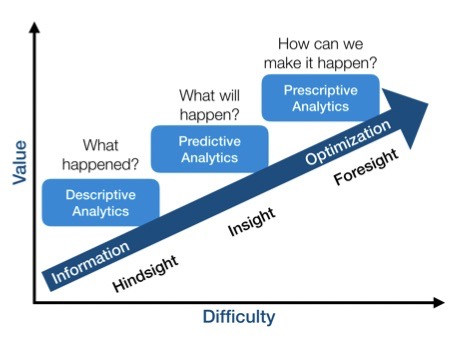
\includegraphics[scale=0.9]{businessAnalytics.jpeg}
\caption{Fasi della business analytics} 
\label{busana}
\end{figure}


% Decisioni
\subsection{Decisioni}

Rappresenta la \hl{scelta di un elemento tra più soluzioni} dopo aver ponderato le opzioni.

Possiamo avere più casi d'uso:
\begin{itemize}
	\item \hl{simplest case}: abbiamo \textbf{poche alternative} quindi una semplice scelta
	\item \hl{multple criteria}: abbiamo \textbf{più metri di paragone} delle performance, quindi si dovranno tenere in conto:
	
	\begin{itemize}
		\item \textbf{soluzioni migliori} di altre (dette di Pareto)
		\item \textbf{vincoli} dovuti dai clienti o da casi logistici da gestire (es: spedizioni)
		\item ottimizzazioni matematiche
		\item \textbf{conflitti tra i vincoli}
	\end{itemize}
	
	\item \hl{incertezze e rischi}: 
	
	\begin{itemize}
		\item \textbf{decisioni operative}: di \textbf{breve periodo}  \textbf{reversibili} e \textbf{limitate} a "n" persone del team
		
		\item \textbf{decisioni tattiche}: \textbf{coinvolge una parte dell'organizzazione} per un medio periodo
		
		\item \textbf{decisioni strategiche}: di \textbf{lungo periodo}  \textbf{non reversibili} e \textbf{coinvolgono denaro}
		
		\item \textbf{decisioni strutturate}: hanno una \textbf{procedura di risoluzione specifica}
		
		\item \textbf{decisioni non strutturate}: richiedono \textbf{creatività} ed \textbf{esperienza} in un  dato settore
	\end{itemize}
\end{itemize}

\begin{figure}[H]
\centering
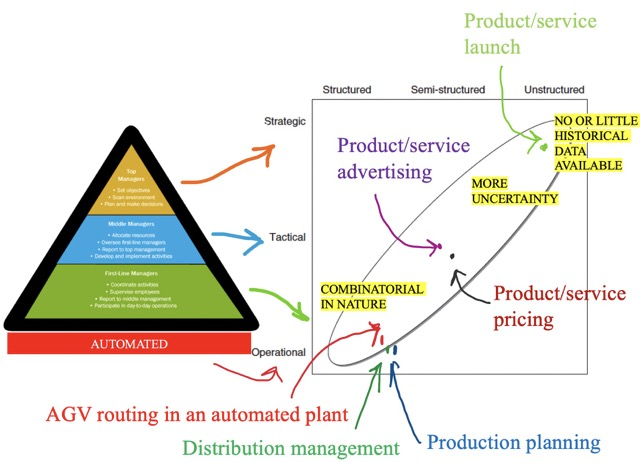
\includegraphics[scale=0.8]{dectax.jpeg}
\caption{Diagonale decisionale} 
\label{diadec}
\end{figure}


% Business Intelligence (BI)
\subsection{Business Intelligence (BI)}

Usato per indicare un \hl{sistema dedicato alla raccolta di dati e alla loro elaborazione} al fine di un reporting, infatti per "Inteligence" si intende investigazione.
Venivano \hl{usati su dati atomici} per avere delle conoscenze approfondite in un determinato business.


% Data visualization
\subsection{Data visualization}

Consiste nel \hl{prendere dati e plottare un grafico}, ma in realtà ora si ha una trattazione più metodologica, cioè se visualizzare in  modo statico o meno i dati.


% Decision Support Systems (DSS)
\subsection{Decision Support Systems (DSS)}

Si indicava un \hl{sistema computerizzato dotato di un sistema di "data managment"} per creare un modello di ottimizzazione, fornendo un feedback tramite un'interfaccia. Ora indica una varietà di sistemi per visualizzare i dati in larga misura o meno.


% Operations Research (OR)
\subsection{Operations Research (OR)}

\hl{Attivita organizzative per portare avanti un sistema logistico}. Per "research" si indica la ricerca delle operation per conseguire dei risultati, avremo come sottocategorie:
\begin{itemize}
	\item \textbf{ottimizzazione matematica}
	\item \textbf{queueing theory}: \textbf{studio matematico delle linee in attesa}  il limite è che funzionano solo con sistemi semplici e con richieste di servizio in ordine stocastico
	\item \textbf{simulazione}: per usarle è \textbf{necessario generare dei numeri randomici}  \textbf{quindi  inconveniente} (bisogna fare un analisi statistica dei risultati dalle quali si farà una \textbf{stima} 
	\item \textbf{game theory}: decisioni con \textbf{più players}
\end{itemize}


% Agents
\subsection{Agents}

È un \hl{sistema che si muove in un environment} (ambiente), ha dei \hl{sensori} tramite i quali percepisce alcuni aspetti del mondo che lo circonda quindi si crea una \hl{rappresentazione del mondo circostante} che può vedere. È capace di \hl{influenzare l'ambiente tramite degli attuatori} come ruote o braccia (intendiamo anche agenti software).

Possiamo classificarli come:
\begin{itemize}
	\item \hl{agenti autonomi}: se è concepito in modo tale che \textbf{tramite un'istruzione sintetica raggiunge un goal sviluppando le azioni per raggiungerlo}  In realtà può anche non essere una sequenza di azioni dato che \textbf{potrebbero esserci degli imprevisti}
	\item \hl{agenti intelligenti}: se
	\item \textbf{impara dall'esperienza}
	\item crea una \textbf{rappresentazione dell'ambiente} che lo circonda e \textbf{ci ragiona sopra} per un possibile risultato delle proprie azioni
	\item \textbf{si adatta ad un ambiente mutevole}
\end{itemize}

\begin{figure}[H]
\centering
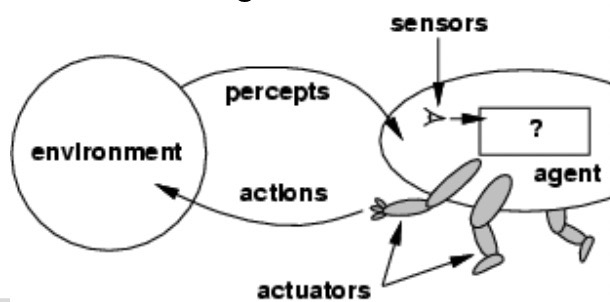
\includegraphics[scale=0.6]{agents.jpeg}
\caption{Schematizzazione di un agente e sue caratteristiche} 
\label{agente}
\end{figure}


% Artificial Intelligence (AI)
\subsection{Artificial Intelligence (AI)}

Comprende tante sottodiscipline:
\begin{itemize}
	\item \hl{automated reasoning}: legato alla \textbf{rappresentazione del mondo} e \textbf{come raggionare su di essa} ma anche calcolandone le probabilità
	\item \hl{automated planning}: usato in ambienti industriali
	\item \hl{automated learning}
	\item \hl{natural language processing}: \textbf{sviluppare agenti software} per fare sintesi di testi, scrivere automaticamente articoli, chat bot, ecc 
	\item \hl{perception}: visione artificiale
	\item \hl{manipuliation}: avere un \textbf{agente che può modificare l'agente} circostante
\end{itemize}


% Machine Learning (ML)
\subsection{Machine Learning (ML)}

Consiste nell'\hl{apprendimento automatico} e quindi lo sviluppo degli \hl{agenti che apprendo tramite la loro esperienza pregressa}. Ci sarà allora una fase di \hl{training}.
Una delle possibili \hl{architetture che permette di farlo sono le Neural Networks} prima avevano solo 2/3 neuroni, ora ne hanno vari strati il che fornisce delle prestazioni impressionanti


% Deep Leaning
\subsection{Deep Leaning}

Si basa sull'\hl{apprendimento automatico} con reti neurale tramite un gran numero di strati di neuroni.


% Data Mining (DM)
\subsection{Data Mining (DM)}

Usare metodi di Machine Learning per \hl{estrarre manualmente dei pattern dai dati}, cioè una \hl{regolarità o un trend}. È quindi la parte nobile del knowledge discovery in db, dato che i dati sono in genere disponibili su db o da altre piattaforme.

La \hl{sequenza} nella quale interviene è:
\begin{enumerate}
	\item \textbf{prendere} i dati
	\item trovare i vari \textbf{target}
	\item \textbf{preprocessare} i dati
	\item trasformare i dati tramite il \textbf{data mining}
	\item trovare dei \textbf{patterns} (dopo il data mining)
\end{enumerate}



































\section{Software solutions and languages for AP and DSS - 29.09.22}


% Decisioni operative/strutturate
\subsection{Decisioni operative/strutturate}

Sono una classe importante, \hl{si possono prendere tramite una procedura standard} che può seguire un manuale o delle normative, automatizzata o no. Queste decisioni di breve periodo si collocano in basso a destra in figura  \ref{diadec}.

Non essendo decisioni dove possiamo solo supportare, allora si possono andare a \hl{codificare in un linguaggio di programmazione procedurale} come C++, Java, ecc...

Potremo avere un \hl{approccio}:

\begin{itemize}
	\item \hl{procedurale}: dove devo far \textbf{generare delle azioni} in seguito di un obiettivo
	
	\item \hl{dichiarativo}: si divide in:
		\begin{enumerate}
			\item \textbf{modellazione} del problema
			
			\item \textbf{descrivo tramite un linguaggio di modellazione} (modelling language) che è un linguaggio di programmazione matematico come AMPL, oppure in linguaggi come python con Amply e Pulp
			
			\item \textbf{solver of the shelf}, che ci darà delle istruzioni per il nostro contesto
		\end{enumerate}
\end{itemize}


\begin{figure}[H]
\centering
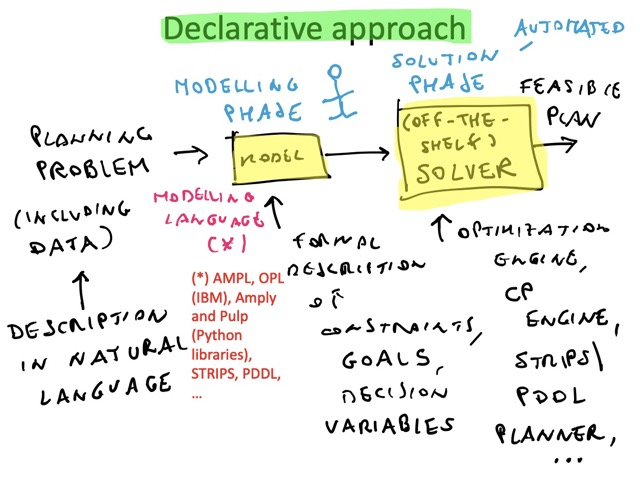
\includegraphics[scale=0.8]{descapp.jpeg}
\caption{procedura implementata} 
\label{descapp}
\end{figure}


Il che è utile dato che \hl{per agire su un problema basterà cambiare il modello} senza cambiare solver, dovrò solo cambiare il modello. È la soluzione più \hl{economico e flessibile} ma è \hl{meno performante} se in ambienti realtime devo prendere soluzioni in tempi molto stretti. Quindi in questi casi servono approcci procedurali.

Per sistemi che devono prendere soluzioni nel breve, si usa \textbf{C, C++, C#}.


% Decisioni non strutturate
\subsection{Decisioni non strutturate o destrutturate}

In questo caso \hl{non possiamo automatizzare}, quindi:

\begin{enumerate}
	\item tiro fuori i \textbf{dati aggregati}
	\item si creano statistiche con \textbf{modelli di ottimizzazione}
\end{enumerate}

Si usano degli \textbf{spreadsheet} che però non riescono a gestire big data e tendono a generare errori.

Il linguaggio più usato è \textbf{Python} ma non è la soluzione più efficiente per tutte quelle applicazioni dove il tempo di calcolo è importante.


% Decisioni semistrutturate
\subsection{Decisioni semistrutturate}

Vogliamo solo \hl{valutare le prestazione di un sistema}. Un esempio sono i sistemi che \hl{presentano un comportamento random} per motivi:

\begin{enumerate}
	\item i \textbf{server hanno un tempo di risposta} che possiamo modellare
	\item le richieste del sistema \textbf{arrivano in maniera stocastica}
\end{enumerate}

Si usano, in questo caso, \hl{metodi simulativi} tramite dei Visual Interactive Modellling System, \hl{per simulare la rete} per la quale passano le informazioni e i server ognuno con diverse proprietà di ciascun linker.



\newpage
\section{Introduzione all'ottimizzazione matematica - 30.09.22}

% Introduzione
\subsection{Introduzione}

Partiamo da un \hl{insieme di formule ed equazioni che modelleranno il problema}. Con questo modello proviamo a trovare una \hl{soluzione} al nostro problema \hl{attraverso algoritmi o risolutori}. L'output è una soluzione per il nostro modello da implementare nel mondo reale.


% Ingredienti principali
\subsection{Ingredienti principali}

Gli ingredienti principali sanno:

\begin{itemize}
	\item \textbf{dati} del problema
	\item variabili: dette anche var decisionali: scelte da fare in merito al problema. rappresentano quindi le scelte, quello su cui il decisore può intervenire
	\item vincoli: equazioni che definiscono i valori che le variabili possono assumere
	\item funzione obietivo: sarà una formula che rappresenta una misura di tipo quantitativo per capire quando è buona la soluzione che abbiamo ottenuto. quindi dovremo ottimizzare questo valore in base al contesto
\end{itemize}


Parleremo di \hl{programmazione lineare con modelli matematici} o relazioni lineari, dato che \hl{molti problemi reali si rifanno a modelli lineari}, per quanto essi possano essere complessi.


% Descrizione del problema
\subsection{Descrizione del problema}

Proviamo a risolvere un problema di mix di produzione, cioè un sistema con un impianto con 2 stabilimenti in cui:

\begin{enumerate}
	\item nel primo: diamo le materie prime e vengono realizzati i componenti in uscita
	\item nel secondo: diamo i componenti realizzati che vengono assemblati per creare il prodotto finito
	\end{enumerate}


\begin{figure}[H]
\centering
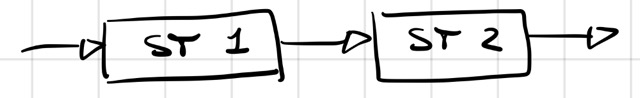
\includegraphics[scale=0.3]{st12.jpeg}
\caption{Catena tra i due stabilimenti} 
\label{st12}
\end{figure}


Supponendo di voler realizzare 2 prodotti A, B con un differente profitto. Determinare il \hl{mix di produzione}, cioè quante unità di A e B produrre la prossima settimana.
Saranno presenti dei \hl{vincoli} creati dalle risorse come i macchinari o gli addetti che potranno lavorare un numero di ore finito.


% Dati del problema
\subsection{Dati del problema}

\begin{itemize}
	\item ore di lavoro:

	\begin{table}[h!]
		\begin{center}
			\begin{tabular}{|c | c c c|} 
 				\hline
 				Stab & A & B & Addetti \\ [0.5ex]
 				\hline
	 			1 & 4 ore & 2 ore & 10 \\
 				2 & 2 ore & 4 ore & 10 \\
				\hline
			\end{tabular}
		\end{center}
		\caption{Tabella delle ore di lavoro}
		\label{taborelav}
	\end{table}

	\item ogni addetto lavora 40 ore/settimana
	
	\item profitto €/pallet:
	
	\begin{table}[h!]
		\begin{center}
			\begin{tabular}{| c c|} 
 				\hline
 				A & B \\ [0.5ex]
 				\hline
 				15k & 10k \\
				\hline
			\end{tabular}
		\end{center}
		\caption{Tabella del profitto €/pallet}
		\label{tabprof}
	\end{table}
	
	\item richiesta del prodotto nella prossima settimana:
	
	\begin{table}[h!]
		\begin{center}
			\begin{tabular}{| c c|} 
 				\hline
 				A & B \\ [0.5ex]
 				\hline
 				40 & 120 \\
				\hline
			\end{tabular}
		\end{center}
		\caption{Tabella del profitto euro/pallet}
		\label{tabprof}
	\end{table}

\end{itemize}


% Descrizione del problema con un modello matematico
\subsection{Descrizione del problema con un modello matematico}

Per \hl{effettuare una modellazione} faremo:

\begin{enumerate}
	\item \hl{identificare le variabili decisionali}:
		\begin{itemize}
			\item $x_A$: \# di pallet di prodotto A da realizzare
			\item $x_B$: \# di pallet di prodotto B da realizzare
		\end{itemize}
		
	\item \hl{definire la funzione obbiettivo (FO)}, per massimizzare il profitto

	\item \hl{definire i vincoli espressi come uguaglianza o disuguaglianza}
		\begin{itemize}
			\item vincolo 1: capacità produttiva dello stab 1 $4x_A+2x_B$ che non può superare $40*10$ cioè ore disponibili ogni settimana per un addetto * numero di addetti: $$4x_A+2x_B <= 400$$
			\item vincolo 2: capacità produttiva dello stabilimento 2 $2x_A+4x_B$ che non può superare $40*10$ cioè ore disponibili ogni settimana per un addetto * numero di addetti: $$4x_A+2x_B <= 400$$
			\item vincolo 3: vincolo sulla richiesta di A: $$x_A <= 40$$
			\item vincolo 4: vincolo sulla richiesta di B: $$x_B <= 120$$
			\item vincolo 5: vincolo di non-negatività: $$x_A, x_B >= 0$$
		\end{itemize}
		
	
\end{enumerate}

	
	
Nella forma completa il \hl{modello complessivo} è:

$$MAX=z=15x_A+10x_B$$

sottoposto ai vincoli (sv):

\begin{itemize}
	\item $4x_A+2x_B <= 400$
	\item $2x_A+4x_B <= 400$
	\item $x_A <= 40$
	\item $x_B <= 120$
	\item $x_A, x_B >= 0$
\end{itemize}


% Risolvere il modello matematico
\subsection{Risolvere il modello matematico}

\hl{Rappresentiamo sul piano cartesiano tutte le soluzioni ammissibili} cercando quella che massimizza il nostro risultato

Impostiamo delle rette per ogni vincolo:

\begin{itemize}
	\item presa $4x_A+2x_B <= 400$ poniamo = 0, a turno, $x_A$ e $x_B$: (200, 100)
	\item presa $2x_A+4x_B <= 400$ poniamo = 0, a turno, $x_A$ e $x_B$: (100, 200)
	\item presa $x_A <= 40$: (40, 0)
	\item presa $x_B <= 120$: (0, 120)
\end{itemize}


Avremo allora una \hl{regione ammissibile} dove valgono tutti i vincoli e nella quale dovrebbe essere presente la nostra soluzione ammissibile. Per trovare il punto che rende massima la funzione $z$ usiamo il \hl{metodo del gradiente}:

$$\nabla z = \left[\begin{array}{c}
	\dfrac{dz}{dx_A}\\
	\dfrac{dz}{dx_B}
\end{array}\right] = \left[\begin{array}{c}
	15\\
	10
\end{array}\right]
$$

dove $\nabla z$ sarà la massima crescita che viene rappresentata tramite (15, 10).

Tracciando una \hl{retta perpendicolare (curve di livello)} alla retta del gradiente avremo valori sempre buoni ma più bassi di quelli sul gradiente, a patto che siano validi. Troveremo in fine il punto massimo che consente di massimizzare, cioè il più estremo alla regione ammissibile sarà il nostro punto.

\hl{Seguendo la retta del gradiente troviamo che la soluzione ottimale} si trova nell'intersezione tra le rette del vincolo 2 con il 3: $x_A = 40$ $2*40+4X_B=400$ quindi $x_B=80$.

La soluzione ottimale sarà:

$$\begin{cases} 
    x_A = 40 \\ 
    2x_A+4x_B = 400
\end{cases}
\begin{cases} 
    x_A = 40 \\ 
    x_B = 80
\end{cases}$$


Si nota che lo stabilimento 2 viene saturato e quello 1 no, dal fatto che la soluzione giace sulla retta del vincolo per il quale si satura.


% Terminologia
\subsection{Terminologia}

Possiamo avere altre forme di modelli di PL:

\begin{itemize}
	\item fo da minimizzare
	\item vincoli di ugualianza
	\item vincoli $>$=
	\item variabili negative
	\item variabili non vincolate
\end{itemize}


Terminologie da sapere:

\begin{itemize}
	\item \hl{soluzione}: quella di output
	\item \hl{soluzione ammissibile}: soluzione, se esiste, che \textbf{soddisfa tutti i vincoli}
	\item \hl{soluzione inammissibile}: se \textbf{viola almeno un vincolo} 
	\item \hl{regione ammissibile}: tutti i punti che rispettano i vincoli
	\item \hl{prob inammissibile}: \textbf{regione ammissibile vuota}
	\item \hl{prob ammissibile}:
		\begin{itemize}
			\item soluzione ottima singola
			\item soluzioni multiple
			\item fo illimitata
		\end{itemize}
\end{itemize}


\begin{figure}[H]
\centering
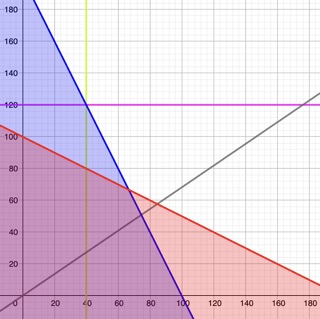
\includegraphics[scale=1]{es.jpeg}
\caption{Rappresentazione grafica esempio} 
\label{rge}
\end{figure}

	
	
% Implementazione in Python
\subsection{Implementazione in Python}

\begin{lstlisting}
import pulp as p

# 1. creazione del modello
model = p.LpProblem("ProductMix", p.LpMaximize)

# 2. definisco le variabili decisionall
x_A = p.LpVariable("x_A", cat="Continuous", lowBound=0)
x_B = p.LpVariable("x_B", cat="LpContinuous", lowBound=0)

# 3. definisco la funzione obiettivo in funzione delle variabili decisionali
model += 15 * x_A + 10 * x_B

# 4. definire i vincoli
model += 4 * x_A + 2 * x_B <= 400
model += 2 * x_A + 4 * x_B <= 400
model += x_A <= 40
model += x_B <= 120

# 5. ricolvere il problema
model.solve()

# print della soluzione
print("next week produce {} pallets of A".format(x_A.varValue))
print("next week produce {} pallets of B".format(x_B.varValue))
\end{lstlisting}


% Esercitazione
\subsection{Esercitazione}

\begin{enumerate}
	\item Massimizzare la f.o. $z = 8x_1 + 6x_2$, con i vincoli:
		\begin{itemize}
			\item $x_1 <= 5$
			\item $x_2 <= 7$
			\item $4x_1 + 3x_2 <= 29$
			\item $x_1, x_2 >= 0$
		\end{itemize}
		
		\begin{figure}[H]
		\centering
		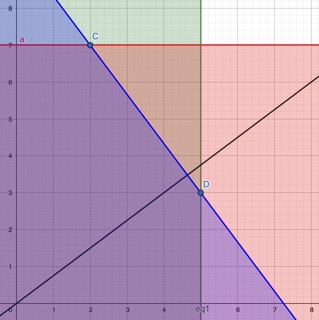
\includegraphics[scale=1]{es1.jpeg}
		\caption{Rappresentazione grafica esempio 1} 
		\label{rge1}
		\end{figure}
		
		$$\nabla z = \left[\begin{array}{c}
			\dfrac{dz}{dx_A}\\
			\dfrac{dz}{dx_B}
		\end{array}\right] = \left[\begin{array}{c}
			8\\
			6
		\end{array}\right]
		$$
		
		\hl{Abbiamo che esiste una curva di livello coincidente con lo spigolo CD, quindi abbiamo delle soluzioni ottime multiple}:
		\begin{itemize}
			\item vertice C, prendiamo allora vincolo 2 e 3:
				$$x_2 = 7 \to x_1 = 2$$
			
			\item vertice D, prendiamo allora vincolo 1 e 3:
				$$x_1 = 5 \to x_2 = 3$$
		
			\item punti del segmento CD
		\end{itemize}
		
		Quindi $z = 58$
	
	
	\item Minimizziamo la f.o. $z = 25x_1 + 22x_2$, con i vincoli:
		\begin{itemize}
			\item $x_1 + x_2 >= 5$
			\item $3x_1 + 2x_2 >= 12$
			\item $3x_1 + 6x_2 >= 18$
			\item $x_1, x_2 >= 0$
		\end{itemize}
		
		\begin{figure}[H]
		\centering
		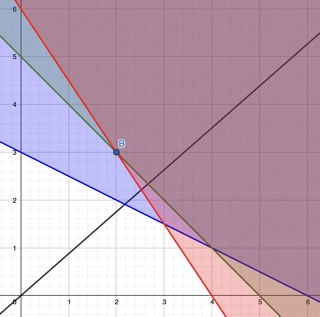
\includegraphics[scale=1]{es2.jpeg}
		\caption{Rappresentazione grafica esempio 2} 
		\label{rge2}
		\end{figure}
		
		$$\nabla z = \left[\begin{array}{c}
			\dfrac{dz}{dx_A}\\
			\dfrac{dz}{dx_B}
		\end{array}\right] = \left[\begin{array}{c}
			25\\
			22
		\end{array}\right]
		$$
		
		Per poter minimizzare, tracciando la curva di livello, trovando che la soluzione ottima si troverà dal punto B dato dall'intersezione dei vincoli 1 e 2:
		$$x_1 = 2, x_2 = 3$$
		
		Quindi $z= 116$
		
	\item Massimizziamo la f.o. $z = 2x_1 + x_2$, con i vincoli:
		\begin{itemize}
			\item $x_1 - x_2 <= 1$
			\item $2x_1 + x_2 >= 6$
			\item $x_2 >= 6$
			\item $x_1, x_2 >= 0$
		\end{itemize}
		
		\begin{figure}[H]
		\centering
		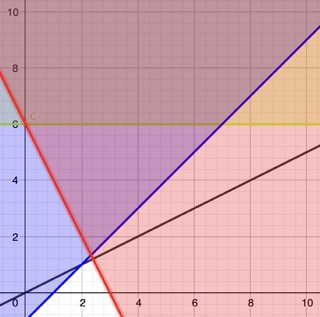
\includegraphics[scale=1]{es3.jpeg}
		\caption{Rappresentazione grafica esempio 3} 
		\label{rge3}
		\end{figure}
		
		$$\nabla z = \left[\begin{array}{c}
			\dfrac{dz}{dx_A}\\
			\dfrac{dz}{dx_B}
		\end{array}\right] = \left[\begin{array}{c}
			2\\
			1
		\end{array}\right]
		$$
		
		\hl{Non raggiungeremo la regione ammissibile, quindi il problema non ammette una soluzione ottima}.
		
	\item Minimizziamo la f.o. $z = -2x_1 + 3x_2$, con i vincoli:
		\begin{itemize}
			\item $x_1 - 2x_2 >= -2$
			\item $2x_1 - x_2 <= 3$
			\item $x_2 >= 4$
			\item $x_1, x_2 >= 0$
		\end{itemize}
		
		\begin{figure}[H]
		\centering
		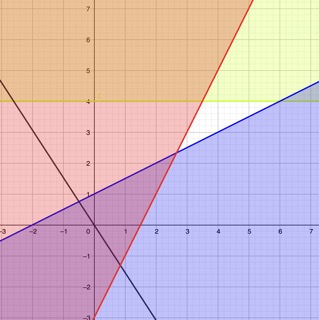
\includegraphics[scale=1]{es4.jpeg}
		\caption{Rappresentazione grafica esempio 4} 
		\label{rge4}
		\end{figure}

		
		$$\nabla z = \left[\begin{array}{c}
			\dfrac{dz}{dx_A}\\
			\dfrac{dz}{dx_B}
		\end{array}\right] = \left[\begin{array}{c}
			-2\\
			3
		\end{array}\right]
		$$
		
		\hl{La regione ammissibile e' vuota e per tanto i problema e' inammissibile, quindi non esiste un punto che soddisfa contemporaneamente tutti i vincoli}.
		
	\item L'azienda vuole decide oltre al piano di produzione anche la giusta riallocazione degli addetti (10-10) tra i due reparti.		
		Le variabili decisionali sono:
		\begin{itemize}
			\item $x_A, x_B$: i prodotti
			\item $n_p$: \# addetti allocati al reparto produzione
			\item $n_a$: \#addetti allocati al reparto assemblaggio
		\end{itemize}
		
		Quindi andremo ad aggiungere il vincolo per cui $n_p + n_a = 20$.
		
		Perciò avremo: $z = 15x_A + 10x_B$, con vincoli:
		\begin{itemize}
			\item $4x_A + 2x_B <= 40n_p$
			\item $2x_A + 4x_B <= 40n_a$
			\item $x_A <= 40$
			\item $x_B <= 120$
			\item $n_a + n_p = 20$
			\item $x_A, x_B, n_a, n_p >= 0$
		\end{itemize}
		

\end{enumerate}











\end{document}
%%%%%%%%%%%%%%%%%%%%%%%%%%%%%%%%
%%%%%% FINE DEL DOCUMENTO %%%%%%
%%%%%%%%%%%%%%%%%%%%%%%%%%%%%%%%




